\documentclass[a4paper,
fontsize=11pt,
%headings=small,
oneside,
numbers=noperiodatend,
parskip=half-,
bibliography=totoc,
final
]{scrartcl}

\usepackage[babel]{csquotes}
\usepackage{synttree}
\usepackage{graphicx}
\setkeys{Gin}{width=.4\textwidth} %default pics size

\graphicspath{{./plots/}}
\usepackage[ngerman]{babel}
\usepackage[T1]{fontenc}
%\usepackage{amsmath}
\usepackage[utf8x]{inputenc}
\usepackage [hyphens]{url}
\usepackage{booktabs} 
\usepackage[left=2.4cm,right=2.4cm,top=2.3cm,bottom=2cm,includeheadfoot]{geometry}
\usepackage[labelformat=empty]{caption} % option 'labelformat=empty]' to surpress adding "Abbildung 1:" or "Figure 1" before each caption / use parameter '\captionsetup{labelformat=empty}' instead to change this for just one caption
\usepackage{eurosym}
\usepackage{multirow}
\usepackage[ngerman]{varioref}
\setcapindent{1em}
\renewcommand{\labelitemi}{--}
\usepackage{paralist}
\usepackage{pdfpages}
\usepackage{lscape}
\usepackage{float}
\usepackage{acronym}
\usepackage{eurosym}
\usepackage{longtable,lscape}
\usepackage{mathpazo}
\usepackage[normalem]{ulem} %emphasize weiterhin kursiv
\usepackage[flushmargin,ragged]{footmisc} % left align footnote
\usepackage{ccicons} 
\setcapindent{0pt} % no indentation in captions

%%%% fancy LIBREAS URL color 
\usepackage{xcolor}
\definecolor{libreas}{RGB}{112,0,0}

\usepackage{listings}

\urlstyle{same}  % don't use monospace font for urls

\usepackage[fleqn]{amsmath}

%adjust fontsize for part

\usepackage{sectsty}
\partfont{\large}

%Das BibTeX-Zeichen mit \BibTeX setzen:
\def\symbol#1{\char #1\relax}
\def\bsl{{\tt\symbol{'134}}}
\def\BibTeX{{\rm B\kern-.05em{\sc i\kern-.025em b}\kern-.08em
    T\kern-.1667em\lower.7ex\hbox{E}\kern-.125emX}}

\usepackage{fancyhdr}
\fancyhf{}
\pagestyle{fancyplain}
\fancyhead[R]{\thepage}

% make sure bookmarks are created eventough sections are not numbered!
% uncommend if sections are numbered (bookmarks created by default)
\makeatletter
\renewcommand\@seccntformat[1]{}
\makeatother

% typo setup
\clubpenalty = 10000
\widowpenalty = 10000
\displaywidowpenalty = 10000

\usepackage{hyperxmp}
\usepackage[colorlinks, linkcolor=black,citecolor=black, urlcolor=libreas,
breaklinks= true,bookmarks=true,bookmarksopen=true]{hyperref}
\usepackage{breakurl}

%meta
%meta

\fancyhead[L]{Redaktion LIBREAS\\ %author
LIBREAS. Library Ideas, 43 (2023). % journal, issue, volume.
\href{https://doi.org/10.18452/27066}{\color{black}https://doi.org/10.18452/27066}
{}} % doi 
\fancyhead[R]{\thepage} %page number
\fancyfoot[L] {\ccLogo \ccAttribution\ \href{https://creativecommons.org/licenses/by/4.0/}{\color{black}Creative Commons BY 4.0}}  %licence
\fancyfoot[R] {ISSN: 1860-7950}

\title{\LARGE{Editorial \#43: Soziologie der Bibliothek}}% title
\author{Redaktion LIBREAS} % author

\setcounter{page}{1}

\hypersetup{%
      pdftitle={Editorial \#43: Soziologie der Bibliothek},
      pdfauthor={Redaktion LIBREAS},
      pdfsubject={LIBREAS. Library Ideas, 43 (2023).},
      pdfkeywords={Soziologie, Bibliothekswissenschaft, Bibliothekswesen},
      pdflicenseurl={https://creativecommons.org/licenses/by/4.0/},
      pdfcopyright={CC BY 4.0 International},
      pdfcontacturl={http://libreas.eu},
      pdfurl={https://doi.org/10.18452/27066},
      pdfdoi={10.18452/27066},
      pdflang={de},
      pdfmetalang={de}
     }



\date{}
\begin{document}

\maketitle
\thispagestyle{fancyplain} 

%abstracts

%body
Bibliotheken sind Teil der Gesellschaften, in denen sie betrieben
werden. Sie sind damit auch Teil der jeweils diese Gesellschaften
prägenden Strukturen, Entwicklungen und sozialen Veränderungen.
Soziologie als Wissenschaft zielt darauf ab, solche gesellschaftlichen
Strukturen zu verstehen und kann somit dazu beitragen, auch die
Entwicklungen in, zu und von Bibliotheken besser zu verstehen. Dies war
die These hinter dem Call for Papers dieser Ausgabe. Hinter dieser stand
stand wiederum die Wahrnehmung, dass es wieder einmal an der Zeit wäre,
darüber nachzudenken, wie soziologische Forschungen, Erkenntnisse und
Methoden in Bezug auf Bibliotheken genutzt werden können.

Erwartungsgemäß ist es nicht das erste Mal, dass das Bibliothekswesen
auf die Soziologie zurückgreift: Im Laufe der letzten 150 Jahre geschah
dies immer wieder und vor allem dann, wenn sich die Gesellschaften
radikal änderten. Als sich beispielsweise die Moderne als
Gesellschaftsdispositiv Ende des 19. und Anfang des 20. Jahrhunderts
durchsetzte, fanden soziologische Theorien über Prozesse der
Urbanisierung, der Entstehung des Massenmarktes und der
Arbeiter*innenschaft ihren Weg in die bibliothekarische Literatur.
Genauso wurde im Bibliothekswesen auf die Soziologie zurückgegriffen,
als nach dem Ersten Weltkrieg mit der Weimarer Republik und der Ersten
österreichischen Republik neue Demokratien im DACH-Raum entstanden und
Bibliotheken versuchten, sich in diesen zu orientieren. Als Ende der
1960er und Anfang der 1970er Jahren eine Welle von gesellschaftlicher
Liberalisierung, Demokratisierung und auch revolutionärem Aufbegehrens
durch die europäischen Staaten ging, war es erneut die Soziologie, von
der sich Bibliotheken versprachen, zu erfahren, was dies alles für sie
bedeutete. Und als sich in den 1990er Jahre der Beginn einer neuen,
marktwirtschaftlichen Epoche abzeichnete, gab es ebenfalls Rückgriffe
auf die Soziologie oder zumindest auf deren Methoden. Dazwischen
allerdings lagen auch immer Jahrzehnte, in denen das Bibliothekswesen
ohne expliziten Rückgriff auf die Soziologie seinen Weg ging -- was, wie
sich zeigte, durchaus funktionsgemäß erfolgreich war. Wo Gesellschaften
mehr oder weniger stabil erscheinen, rückt der Bedarf einer expliziten
Gesellschaftsanalyse anscheinend in den Hintergrund.

Aktuell scheint es so, als gäbe es gute Gründe, sich wieder einmal der
Soziologie im Zusammenhang mit Bibliotheken zuzuwenden. Denn
zweifelsohne (und auch ohne Blick auf das Zuspitzungs- und
Konfrontationsmedium Twitter) werden massive Verschiebungen und
Verwerfungen sichtbar. Sie beginnen im politischen und öffentlichen
Diskurs und wirken zurück auf politische, kollektive und individuelle
Entscheidungen und Handlungen. Die zwei auseinander driftenden
Grundlinien sind erkennbar einerseits eine Entwicklung hin zu mehr
Diversität und Offenheit und andererseits ein neuer Aufschwung des
Autoritarismus. Nicht nur weil sich nahezu jede Verästelung dieser
Debatte früher oder später in Büchern wiederfindet, drängen diese
Spannungen in die Bibliotheken. Aber natürlich ist der Bestandsaufbau
hier auch ein Thema.

Gleichzeitig setzt sich gerade im Öffentlichen Bibliothekswesen die Idee
durch, dass den Bibliotheken neue, gesellschaftliche Funktionen zukommen
würden, für die sie umgebaut und ihre Aufgabenbereiche erweitert werden
müssten. Sie sind Schauplatz und Vollzugsort von Öffentlichkeit,
kultureller und, Stichwort Makerspaces, auch aktiver Arbeit. Darüber
kann und sollte man bibliothekssoziologisch forschen. Nur: Wer macht's?

\begin{figure}
\centering
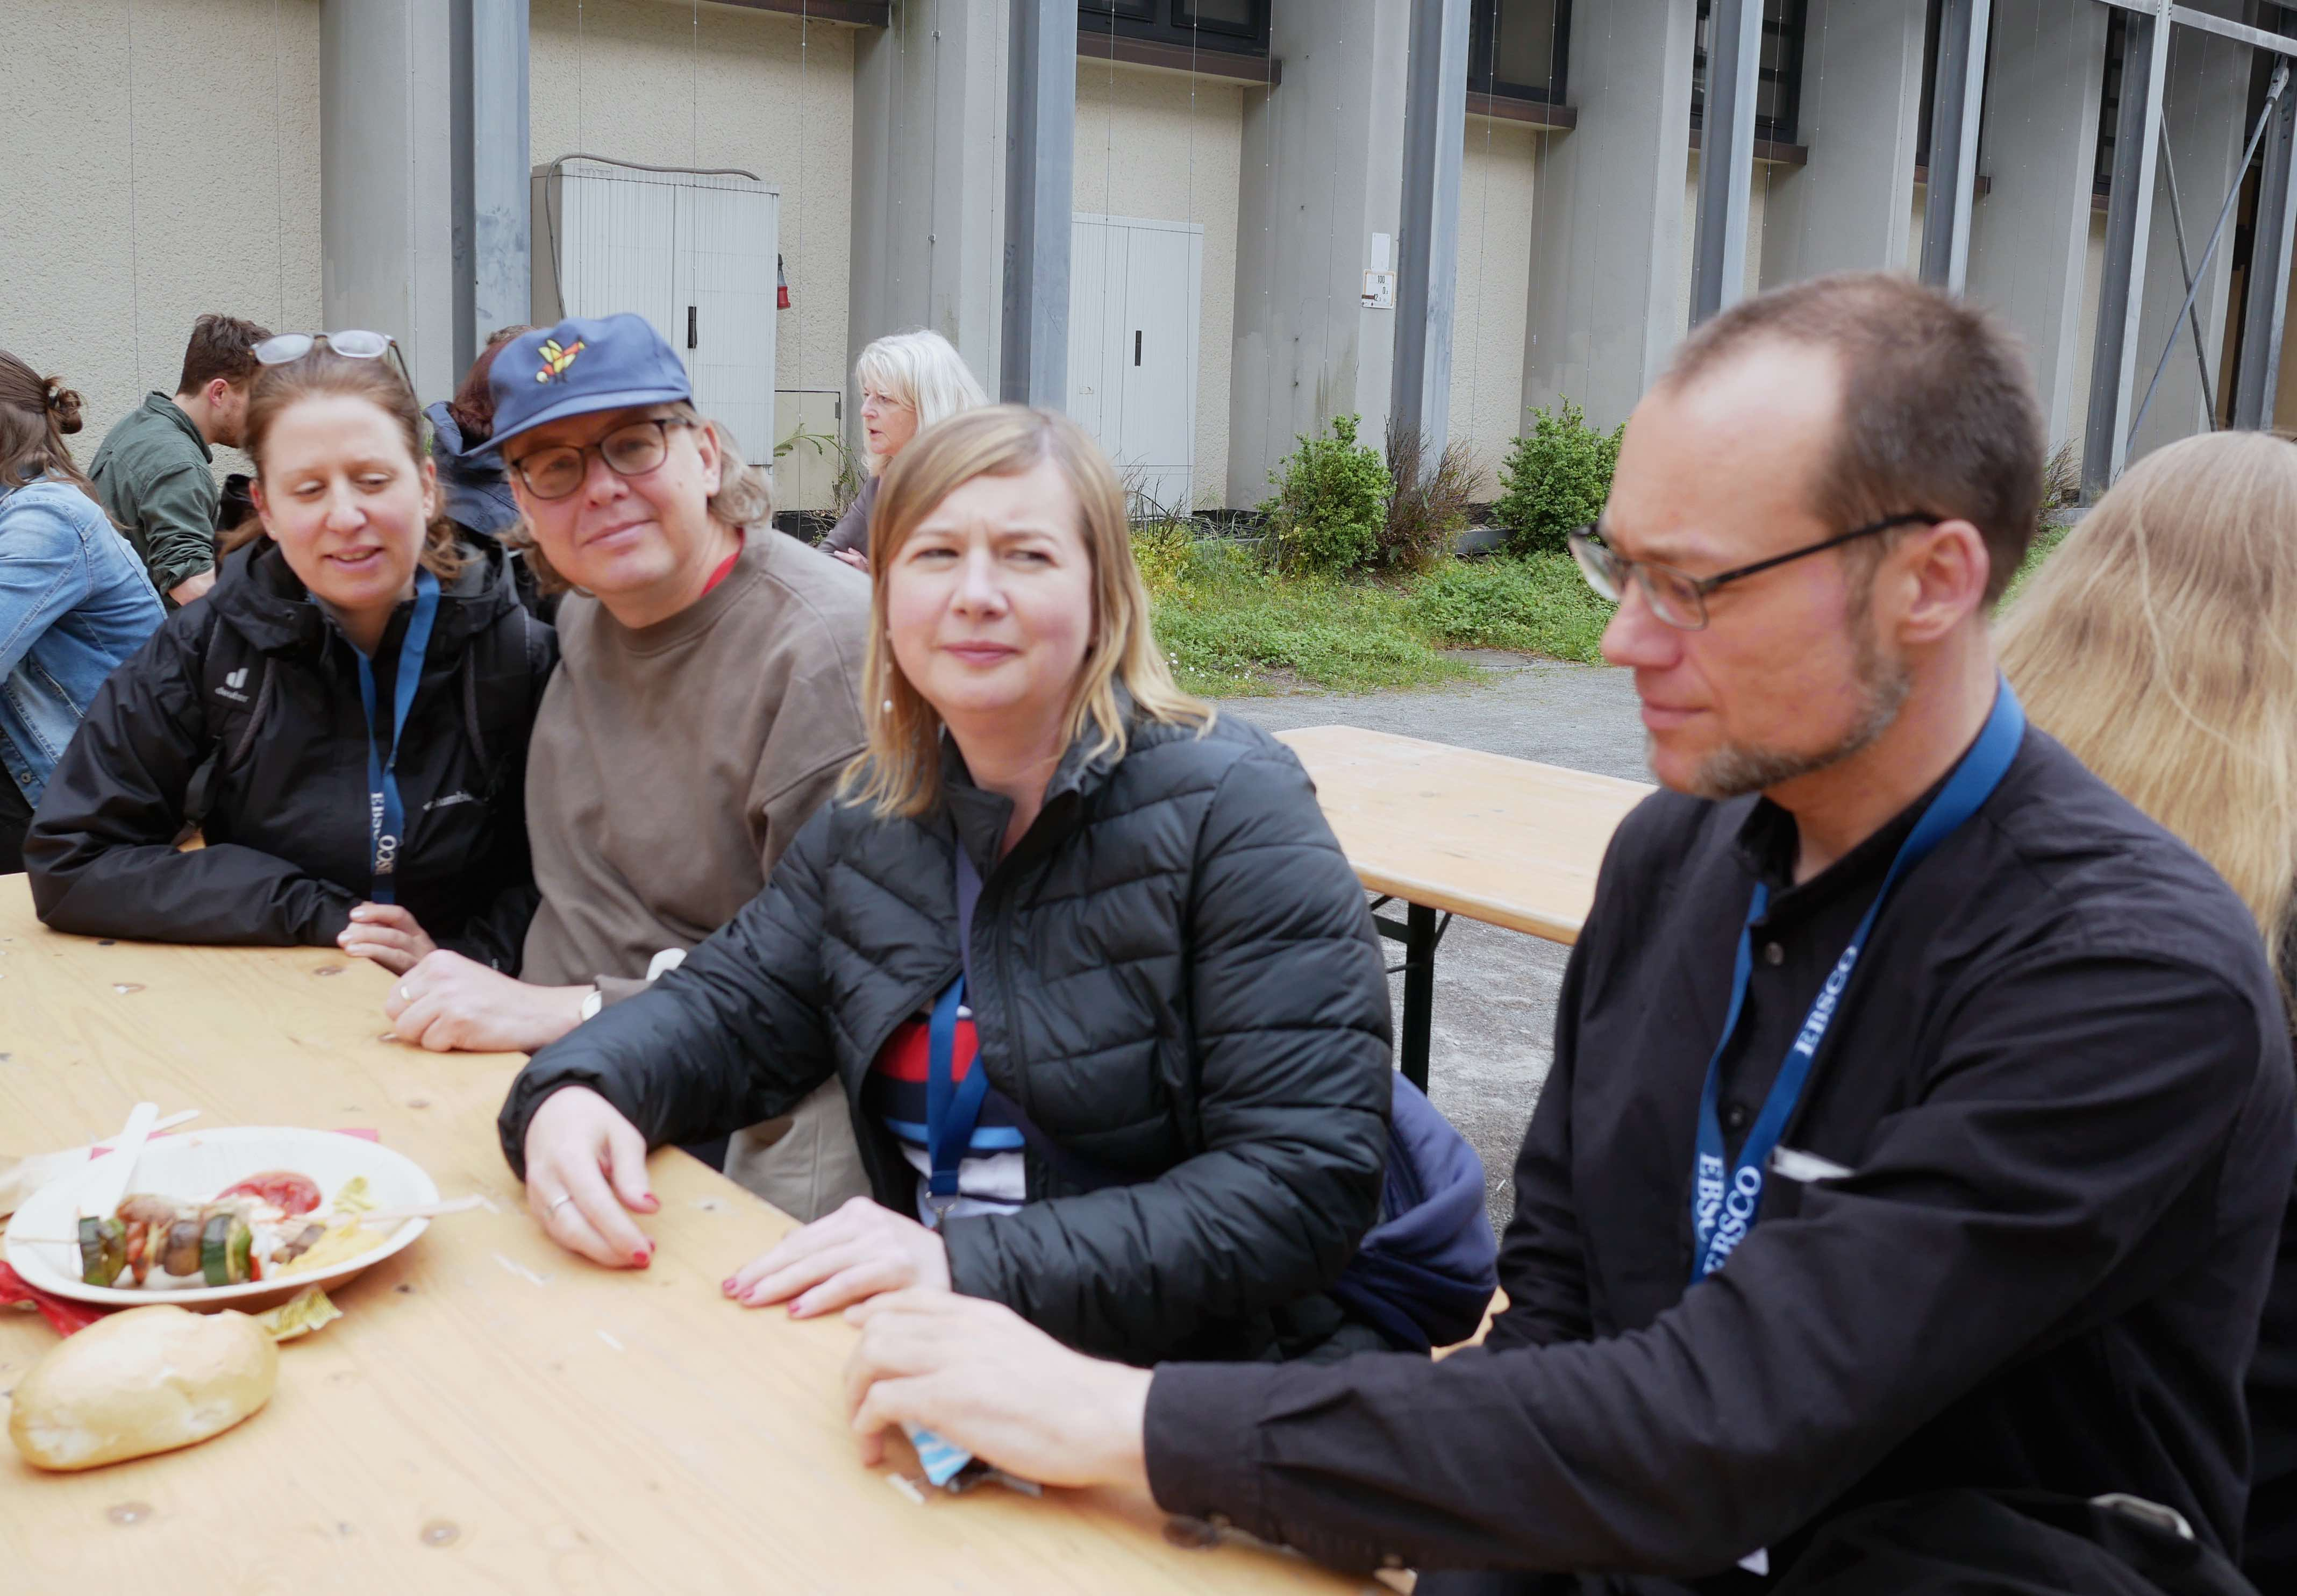
\includegraphics[width=0.5\textwidth]{editorial.jpg}
\caption{Redaktionsorte XXII: Hannover Congress
Centrum, beim Grillstand, Frühling 2023}
\end{figure}

De Beteiligung an und Rückmeldungen zu dieser Ausgabe zeigen uns, dass
eine Bibliothekssoziologie nicht unbedingt das zugkräftigste Stichwort
ist. Die drei eingegangenen Beiträge nutzen soziologische Theorien und
Methoden und zeigen also, dass es sehr gut möglich ist, diese mit
relevanten Ergebnissen auf Bibliotheken und deren Themen anzuwenden.
Aber gleichzeitig scheinen sich nicht viele Kolleg*innen aktiv mit der
Soziologie zu befassen. Oder sind die gesellschaftlichen Veränderungen
vielleicht gar nicht drängend, wie sie beispielsweise um 1900 schienen?
Oder laufen Elemente soziologischer Erkenntnisfindung sublimiert in
jeder Bibliothekswissenschaft einfach mit? Oder ist LIBREAS als
Publikationsort nicht attraktiv genug? Fakt ist, dass auch die
einschlägigen Nachweissysteme zu wenig aktueller Literatur führen, die
sich explizit als bibliothekssoziologisch positioniert.

Hätten wir, als wir uns für das Thema dieser Ausgabe entschieden, eher
auf Entwicklungen im Bereich Social Media und Artificial Intelligence
(AI) gesetzt, wir hätten jetzt vermutlichl ein umfangreicheres Heft --
möglicherweise inklusive zahlreicher ChatGPT-generierter Inhalte. In
beiden Bereichen gab es seit unserer letzten Nummer Aufsehen erregende
Bewegungen. Social Media ist Post-Elon-Musk genauso neu zu denken wie
Konzepte von Kreativität und Autor*innenschaft nach der Bereitstellung
massentauglicher KI-Tools. Twitter nach Elon Musk bedeutet, so scheint
es aktuell, früher oder später auch ein Twitter ohne Bibliotheken. Denn
welches Haus hat schon Kapazitäten und Lust, den Sturm der rohen,
ungefilterten Entrüstung zu moderieren, der sich unweigerlich
beispielsweise bei der Ankündigung einer Lesung mit Dragqueens ergibt.
\enquote{Trigger} sind ein fantastisches neues Forschungsfeld der
Sozialpsychologie und die Hölle für die, die es trifft. Bibliotheken
sehen sich entsprechend lieber bei Mastodon. Aber sehen sie dort auch
ihr Publikum? Oder warten alle auf Bluesky?

Und was machen wir zugleich mit KI-generierten Inhalten? Neulich, zu
spät für die Rubrik \enquote{Das liest / hört die LIBREAS}, erfuhr
mensch im Deutschlandfunk von der Zukunft der Filmkultur: Sven Bliedung,
CEO der Videoinnovationsfirma Volucap, prophezeite, dass wir binnen
weniger Jahre befähigt sein sollen, uns per Eingabe von Keywords oder
gar Stimmungen ein KI-generiertes Filmprogramm in Echtzeit zu
generieren: \enquote{Man kommt nach Hause, hat einen stressigen Tag
gehabt, macht einen Bildschirm an, will unterhalten werden, und
{[}...{]} braucht kein Programm auswählen, weil das System weiß, was ich
für einen Tag hatte, ob ich irgendwie Entspannung suche oder Action und
es wird automatisch eine Geschichte geschrieben und die Bilder dazu
erzeugt.}\footnote{Berendt, Christian: Virtuelle Drehorte -- Wie das
  Filmstudio Babelsberg mit KI arbeitet, Deutschlandfunk 11. Mai 2023,
  \href{https://www.deutschlandfunk.de/virtuelle-drehorte-wie-das-filmstudio-babelsberg-mit-ki-arbeitet-dlf-a796598c-100.html}{https://www.deutschlandfunk.de/virtuelle-drehorte-wie-das-filmstudio-babelsberg-mit-ki-arbeitet-dlf-a796598c-100.html}}

Was das nicht nur mediensoziologisch bedeuten würde, ist noch ein ganz
anderes Thema und würde eine eigene KI-Simulation eines Textes von
Jean-Louis Baudry zum Dispositiv automatisch erstellter Filme nahezu
erzwingen.

Akuter greift sicher die KI-gestützte Textproduktion in Forschung und
Lehre. Universitätsbibliotheken sehen sich zunehmend genötigt, in Kursen
zum wissenschaftlichen Arbeiten neben der Plagiatserkennung auch
Kompetenzen zum Erkennen von per KI identifizierten oder eben auch
erfundenen Quellen zu vermitteln.

Als wir die vorliegende Ausgabe planten, waren noch Dienste wie DeepL
und Transkribus die Vorzeigebeispiele für die Möglichkeiten solcher
Technologien, jetzt sind schon ganze Zeitungsredaktionen verkleinert
worden, weil die Eigentümer*innen den Eindruck haben, Journalist*innen
ersetzen zu können. Diese Entwicklungen zeigen aber, wie schnell sich
Dinge ändern, an die bei der Planung von Zeitschriften und Artikeln
nicht gedacht wird. Sind wir gespannt auf den Rest des Jahres 2023.

Um es für diese Ausgabe abzurunden, baten wir ChatGPT, ein paar Gründe
für den wahrgenommenermaßen geringen Stellenwert der
Bibliothekssoziologie zu extrahieren. Das Ergebnis deckt sich
erstaunlich gut mit dem, was wir aus dem Bauch heraus vermuten würden:

\begin{enumerate}
\def\labelenumi{\arabic{enumi}.}
\item
  Bibliotheksforschung ist traditionell auf die \enquote{Entwicklung von
   Bibliotheksmethoden, -technologien und
  -dienstleistungen} und  deren praktischer Umsetzung
  ausgerichtet.
\item
  Bibliothekssoziologie ist ein interdisziplinäres Forschungsfeld,
   wobei dieser Status nicht zu einer Forschung von beiden
  Seiten  sondern zu einer Marginalisierung dieser Themen
  auf beiden Seiten  führt.
\item
  Ressourcen: \enquote{Da bibliothekarische Institutionen oft mit
  begrenzten  Budgets arbeiten, können Forschungsprojekte
  im Bereich der  Bibliothekssoziologie möglicherweise
  nicht die erforderliche  Unterstützung erhalten, um
  umfangreiche und aussagekräftige  Studien
  durchzuführen.}
\item
  Geringe Nachfrage: \enquote{Bibliothekare und Entscheidungsträger
   konzentrieren sich möglicherweise eher auf praktische
  Fragen wie  die Verbesserung der Dienstleistungen, der
  technologischen  Infrastruktur oder der
  Ressourcenallokation, anstatt auf  soziologische Aspekte
  der bibliothekarischen Arbeit.}
\end{enumerate}

Wie gern hätten wir auf die Quelle verlinkt. Allerdings bleibt die
Vergabe eindeutiger Links, also PID für mit ChatGPT generierte Inhalte
auch Monate nach dessen Einführung ein Desiderat. Wir behalten es aber
im Blick und berichten gegebenenfalls in der Herbstausgabe über
entsprechende Neuerungen.

Ihre / eure Redaktion LIBREAS. Library Ideas

(Berlin, Göttingen, Hannover, Lausanne, München, Potsdam)

%autor

\end{document}